\documentclass[oneside, 12pt]{ctexart}

\usepackage[left=2cm, right=2cm, top=2.5cm, bottom=2.5cm]{geometry} %margin设置

\usepackage{amsmath}
\usepackage{amssymb}
\usepackage{mathtools}
\usepackage{amsthm}
\usepackage{listings}
\usepackage{tikz-cd}
\usepackage{float}

\newtheorem{definition}{定义}[section]
\newtheorem{property}{性质}[section]
\newtheorem{proposition}{命题}[section]
\newtheorem{theorem}{定理}[section]
\newtheorem{remark}{评价}[section]
\newtheorem{example}{例}[section]

\author{zysx997}
\title{后继结构}

\begin{document}

\maketitle

\section{认识数,从认识数数开始}

原本打算把标题起成“认识数学,从认识数数开始的”,但仔细一想不太合理。如果想要认识自然数,从数数开始是很有必要性的。但是对于整个数学,或许认识集合、认识范畴、认识泛性质才是最为重要的。正如接下来我在处理“数数”的问题中,多次用到集合、范畴、泛性质的工具。这些工具或许不是必要的,但往往能解释清楚我们进行构造的动机,或是构造的原因。因此,认识这些概念是有益的,从“数数”这个简单的例子开始,用来辅助理解这些概念也是有帮助的。

我认为数学中定义一种结构的抽象有两个方面。一是把现实中或者概念中的直觉用数学的语言描述,给出一个“基础”,二是利用逻辑推理,在基础上附加更多“良好”的性质,以便我们对结构进行处理。在这个观点下,让我们来看看数学中是怎么对自然数进行抽象的。首先,自然数对应的现实直觉来自“数数”,运用集合代数的知识,我们可以将“自然数集”抽象为一个集合$\mathbb{N}$,然后,将“数数”这个操作定义为一个从$\mathbb{N}$到其自身的映射$s$。这样,我们就把自然数的定义从“数数”这个操作抽象为一个集合上的映射。这一步的抽象是很自然的,因为我们知道,自然数是一个集合,而“数数”这个操作就是把集合中的元素按照一定的顺序取出来。这个操作可以被抽象为一个映射。然而,我们并没有定义这个映射,也没有给出这个映射的性质。这就是我们需要进行的第二个步骤。我们需要定义这个映射,或是给出这个映射的性质。这个映射的定义或性质的给出,就是我们需要进行的第二步抽象。如果熟悉Peano公理,那么你应该会明白,Peano公理的几条性质就是第二步抽象的结果。在这里我们先列出自然数集$\mathbb{N}$与后继映射$s \colon \mathbb{N} \to \mathbb{N}$满足的Peano公理:

\begin{description}
	\item[Zero]
		\begin{gather*}
			0 \in \mathbb{N}
		\end{gather*}
	\item[Zero is not a successor]
		\begin{gather*}
			\mathop{\forall}\limits_{n \in \mathbb{N}} ns \not= 0
		\end{gather*}
	\item[Injective]
		\begin{gather*}
			\mathop{\forall}\limits_{m,n \in \mathbb{N}} ms = ns \rightarrow m = n
		\end{gather*}
	\item[Induction]
		\begin{gather*}
			\mathop{\forall}\limits_{A \subset \mathbb{N}} (0 \in A \wedge (\mathop{\forall}\limits_{n \in \mathbb{N}} n \in A \rightarrow ns \in A)) \rightarrow A = \mathbb{N}
		\end{gather*}
\end{description}

注意,在上面的符号中我们对$n$在映射$s$下的像记为$ns$,而不是$s(n)$。这样做是为了符合我们从左向右书写的习惯。另外,上面列出的Peano公理说没有包括$ns \in \mathbb{N}$这一条,因为$s$作为$\mathbb{N} \to \mathbb{N}$的函数,已经包含了这个性质。注意,Peano公理的Zero条目并非关于映射$s$,而是关于集合$\mathbb{N}$。因此,自然数集的基石与其说是集合$\mathbb{N}$与映射$s$两者,不如说是集合$\mathbb{N}$、映射$s$与元素$0$三者。而在这三者的基础上,进一步应满足Peano公理的Zero is not a successor、Injective与Induction三条性质。但是,除了抽象的第一步对$s$的定义,再加上$0$作为某个“起点”符合我们对于“数数”直觉的抽象之外,我们并不知道剩下的三条性质是如何与我们关于“数数”的直觉相联系的。或许更好的问法是:具有一个确定点$x$,一个自映射$s$的集合$X$有很多,为什么我们偏偏对于满足上面的三条性质的有确定点$0$,自映射$s$的集合$\mathbb{N}$感兴趣?这个问题,更一般的问法,是“一个结构的全体中有那么多结构对象,为什么会有一些特殊的结构对象,我们特别感兴趣?”。这个问题的解答,其主观成分在于“我们对怎样的数学对象感兴趣”,而客观成分在于,当我们确定了对怎样的数学对象兴趣后,我们能严格地证明,某些性质是这些数学对象的必然性质。这就是数学的魅力所在。

让我们来先对主观成分进行讨论。我们会对怎样的数学对象感兴趣呢?首先,这里要澄清一点,这里的数学对象是来自已经定义了的结构全体的,而这样的结构全体的定义来源于直觉,是上面说的第一步抽象。已经定义的某个结构全体,其可以有各种各样不同的结构对象,我们最为关注的是能反映所有对象性质的那些特别的对象。举例明之,如果结构全体是一个闭区间,对象是其中的元素,那么我们最关注的对象自然是最大元$b$与最小元$a$,因为如果确定了这两者,那么所有其他的元素都得到了确定。在这里,我们用特殊的两个对象,得到了关于全体对象的性质。像这样关于全体对象的性质,称为这个结构的泛性质。一个对象能反映结构的泛性质,是我们对这个对象感兴趣的主要原因。这里要说明的是,对象之所以能反映整个结构的泛性质,是因为这个对象与结构的其他对象之间有着联系,这种联系也是结构必须含有的一部分,不然的话,结构中的对象就是孤立的,没有联系,也就不可能用一个对象反映整个结构的性质。

关于问题的客观成分,需要用到范畴论。范畴论是系统地研究结构、关系、泛性质的理论。范畴论是数学的一种基础理论,它研究的是数学对象之间的关系,以及这些关系的性质。范畴论的基本概念是范畴,一个范畴包括了对象、态射与态射的复合。对象是我们研究的数学对象,态射是对象之间的联系,这种联系可以通过复合进行传递。有了范畴提供了关于结构、对象、关系的统一语言,我们就可以证明某些对象在某种意义下的唯一性,这就得到了这样的数学对象的“必然性质”。接下来,一旦确定了对象和联系的定义,我们就会用“范畴”代替“结构全体”,用“对象”代替“结构对象”,用“态射”代替“联系”,作为更标准的术语。

让我们回到关于自然数的问题。我们由第一步抽象,得到一种具有一定结构的对象:一个集合$X$,具有一个自映射$s$,同时具有一个确定点$x$。这种结构的对象包含了$3$个特征,或者说属性,我们用$3$元组方便地表示它,记为$(X, s, x)$。这里使用$X$与$x$作为符号而不使用$\mathbb{N}$与$0$的原因是,当我们提及$\mathbb{N}$与$0$时,往往默认了Peano公理,而这里我们考虑的是不一定具有特殊性的结构对象。这样的结构对象,我们就由它的元素构成,叫它“带基点的后继集合”吧。在这里,基点指的是$x$,后继指的是集合$X$上的自映射$s$,我们将其视为一种一元运算,或者也可以叫算子,称为后继算子。有了结构的对象,它们之间还需要相互联系。在集合范畴中,我们定义态射的标准方式是把态射定义为两个集合之间的映射。至于集合之间的联系为什么既不是要求更高的单射、满射、双射,又不是更弱的二元关系,这个问题有些意思。
%猜想:范畴论中的范畴也不仅仅是通常的范畴一种,还有添加了更多联系的Abel范畴。那么,我们可以从这个事实得到一个有益的看法:范畴的公理不是锁定的,可以因为研究对象的特殊性而增加,当然应该也能减少。那么,对于映射,我们定义了标准的范畴;对于更强的二元关系如单射、满射,一定也能在标准范畴的框架下处理;但是如果对于更弱的一般二元关系,或许在标准范畴公理下处理起来就不太方便了。这时候我们可能要定义新的范畴。总结一下,上面的猜想回答了“为什么集合范畴的态射是映射”这个问题,它告诉我们映射并不特殊,只是范畴的公理天生就是为映射设计的,而对于其他联系,我们可以定义新的范畴。
不过,我们的标准做法依然是把集合间的态射定义为映射。而我们在此处考虑的带基点的后继集合,它本质上是在一个集合上附加了两个结构:一个自映射与一个基点。因此,我们一方面继承集合范畴的态射,把带基点的后继集合$(X, s, x)$到带基点的后继集合$(X', s', x')$间的态射定义为某种映射$f \colon X \to X'$。另一方面,我们还需要考虑这个映射应该在附加的两个结构上建立联系,或者说如何保持自映射与基点的结构。保持这两个结构的方法很简单,首先是对于基点,保持基点我们能想到的唯一标准方法无非是使$xf = x'$;而对于后继算子,保持运算的标准方法是,考虑$X$中的元素$y, z$满足$ys = z$,我们可以对它在这两个点在映射$f$下得到像$yf, zf$,既然和$X$中$y$可由一步后继得到$z$,那么,我们就想在$X'$中,使像$yf$由一步后继得到$zf$。换言之,我们想让等式$yfs' = zf$对一切满足$ys = z$的$y,z \in X$成立。由于$z$可用$y$代入,这相当于下面的式子成立:
\begin{gather*}
	\mathop{\forall}\limits_{y \in X} yfs' = ysf, \quad \text{即} \quad fs' = sf.
\end{gather*}
实际上,我们可以用交换图来更加直观地展示这个关系:
\begin{center}
\begin{tikzcd}
	X \arrow[r, "f"] \arrow[d, "s"'] & X' \arrow[d, "s'"] \\
	X \arrow[r, "f"'] & X'
\end{tikzcd}
\end{center}
我们的态射定义源于集合映射定义,因此态射的复合可以直接定义为集合映射的复合,单位态射也可直接定义为一个集合的恒等映射。严格地说,为了使这样的定义符合范畴的公理,我们还需验证态射的复合也是态射,以及对单位态射定义本身满足态射的性质。恒等映射符合上面对态射的要求,这一点是显然的,关键在于对态射复合仍为态射的验证。这里我们使用交换图的方式进行直观验证:
\begin{center}
\begin{tikzcd}
	X \arrow[r, "f"] \arrow[d, "s"'] & X' \arrow[r, "g"] \arrow[d, "s'"'] & X'' \arrow[d, "s''"] \\
	X \arrow[r, "f"'] & X' \arrow[r, "g"'] & X''
\end{tikzcd}
\end{center}

于是,我们可以将所有带基点的后继集合作为对象,它们之间满足上面给出要求的映射为态射,得到带基点的后继集合的范畴。我们用$\mathsf{Succ_\bullet}$表示它,其中$\bullet$表示有一个基点。我们再总结上面对$\mathsf{Succ_\bullet}$给出的定义:

\paragraph{范畴$\mathsf{Succ_\bullet}$}
\begin{description}
	\item[对象] 所有带基点的后继集合$(X, s, x)$。
	\item[态射] 从$(X, s, x)$到$(X', s', x')$的态射是一个映射$f \colon X \to X'$,满足$xf = x'$与$fs' = sf$。
	\item[态射的复合] 若$f \colon (X, s, x) \to (X', s', x')$,$g \colon (X', s', x') \to (X'', s'', x'')$,则$f \circ g \colon (X, s, x) \to (X'', s'', x'')$定义为集合映射的复合$f \circ g$。
	\item[单位态射] 对于每个对象$(X, s, x)$,单位态射$\text{id}_{(X, s, x)} \colon (X, s, x) \to (X, s, x)$定义为集合$X$上的恒等映射$\text{id}_X$。
\end{description}

研究这个范畴可以告诉我们自然数所额外满足的性质有什么重要性。不过,对于对象的三部分信息,或者说三部分资料,实际上基点所提供的信息是最少的。因此,我们可以考虑去掉基点,只研究带后继算子的集合。这样的集合,我们称之为“后继集合”。后继集合的范畴的定义与带基点的后继集合的范畴的定义类似,只是去掉了基点的信息。我们将后继集合的范畴记为$\mathsf{Succ}$,并在下面给出它的定义:

\paragraph{范畴$\mathsf{Succ}$}
\begin{description}
	\item[对象] 所有后继集合$(X, s)$。
	\item[态射] 从$(X, s)$到$(X', s')$的态射是一个映射$f \colon X \to X'$,满足$fs' = sf$。
	\item[态射的复合] 若$f \colon (X, s) \to (X', s')$,$g \colon (X', s') \to (X'', s'')$,则$f \circ g \colon (X, s) \to (X'', s'')$定义为集合映射的复合$f \circ g$。
	\item[单位态射] 对于每个对象$(X, s)$,单位态射$\text{id}_{(X, s)} \colon (X, s) \to (X, s)$定义为集合$X$上的恒等映射$\text{id}_X$。
\end{description}

接下来,我们就深入研究范畴$\mathsf{Succ}$的对象的性质,以及该范畴的泛性质。

\section{对后继集合的研究}

\subsection{后继闭集和后继闭包}

现在我们的任务是,对一个一般的后继集合$(X, s)$,研究它的性质。在接下来的讨论中,我们时常会设出一个点$x \in X$,如果我们这么做了,那么我们就默认此时$X$是非空的。请注意这一点。

因为后继集合$X$上有后继算子$s$,我们可以考虑从一个元素$x$出发,对$x$施以$s$的多次作用,得到一系列元素$x, xs, xss, xsss, \cdots$。我们先研究这样的一系列元素,将其放在一个集合中,我们称之为元素$x$的后继闭包,记为$\overline{x}$。
%注意这里我们将$x$记在右边,表示$x$得到的后继子集,但是在表示$x$在映射$s$下的像时,我们将$x$记在左边。这么做的原因是,在表示$x$在映射$s$下的像时,我们是将像作为一个整体考虑的,这时为了使映射的复合符合我们从左向右书写的规则,我们将映射写在右边,将参与映射的元素$x$记在左边;而在表示$x$生成的后继子集时,我们更强调$T_{\bullet}$是一种“抽象的子集”,而将$T_x$看成抽象的子集应用于$x$的结果。这里我们将$T_{\bullet}$与$x$分开来看了,先有了$T_{\bullet}$,再有了应用于$x$得到的$T_x$,所以我们将$x$作为放在右边的下标。
%这一段已经过时,因为采用了闭包的符号,不再需要这样的记号。

然而,上面对$x$的后继闭包的定义并不严谨,什么是集合$\{x, xs, xss, xsss, \cdots\}$?这个集合的元素我们似乎完全无法列举出来。因此,我们在定义$\overline{x}$时,要考虑另一种定义方法:考虑$\overline{x}$应该满足什么性质。我们将$\overline{x}$的性质分为两部分,一是$\overline{x}$包含$x$,二是$\overline{x}$在我们讨论的集合$X$的后继算子$s$下封闭。我们将前者称为Base性质,后者称为Inductive性质。这里,我们其实又在做第一步抽象,其抽象出了$\overline{x}$应满足的性质,然而我们将看到,这个性质不足以唯一地确定一个子集。因此,我们不妨先考虑所有满足这个性质的子集的集合,我们称之为含$x$的后继闭集族,记为$\mathcal{C}_x$,其中$\mathcal{C}$表示“闭集”(closed set)。

注意这里我们是将$x$记在$\mathcal{C}$的右边的。这与我们在表示$x$在映射$s$下的像时将$x$记在左边的原因是一样的。我们将$x$放在右边,是因为我们对每个$x \in X$都能定义$\mathcal{C}_x$,相当于我们有了抽象的集族$\mathcal{C}_{\bullet}$,再将抽象的集族应用于$x$得到具体的集族$\mathcal{C}_x$,所以我们将$x$作为放在右边的下标。这样的记号也是为了使我们的记号符合我们从左向右书写的规则。甚至可以理解为,$x$是一个映射,将$\mathcal{C}_\bullet$映射到$\mathcal{C}_x$,这样的记号也是合理的。

我们接下来将$\mathcal{C}_x$的定义写出来:

\begin{definition}[含$x$的后继闭集族$\mathcal{C}_x$]
	对于后继集合$(X, s)$,$x \in X$,我们定义含$x$的后继闭子集族$\mathcal{C}_x$为满足以下性质的集合$T \subset X$的集族:
	\begin{description}
		\item[Base on $x$] $x \in T$
		\item[Inductive] $\mathop{\forall}\limits_{y \in T} ys \in T$
	\end{description}
\end{definition}

首先要注意一个技术上的细节,我们这样定义出的$\mathcal{C}_x$一定是非空的,这样才能便于我们之后的讨论。这是因为,整个后继集合$X$一定是满足Base与Inductive性质的子集。那么,我们不禁仍要问,我们想要定义的$x$的后继闭包$\overline{x}$,到底是集族$\mathcal{C}_x$中的哪个集合呢?显然,在很多情况下,我们不会希望它是整个后继集合$X$。如果再作思索,我们会发现,我们不想在$\overline{x}$中添加任何不必要的元素。因此,我们希望$\overline{x}$尽量“小”,这里的“小”指的是在包含关系$\subset$下的“小”,确切地说,是包含关系作为集族中的偏序关系下的最小元。事实上,我们可以证明,$\mathcal{C}_x$中的确存在着一个包含关系下的最小元,因此我们将$\overline{x}$定义为这个最小元。具体的论述用到关键性质是“交性质”:

\begin{property}
	对于后继集合$(X, s)$,$x \in X$,$\mathop{T_i}\limits_{i \in I} \in \mathcal{C}_x$,其中$I$为非空指标集,则$\bigcap\limits_{i \in I} T_i \in \mathcal{C}_x$。
\end{property}

\begin{proof}
	首先,由于$\mathop{T_i}_{(i \in I)} \in \mathcal{C}_x$,即对于每个$\mathop{\forall}_{(i \in I)}x \in T_i$,有$x \in \bigcap_{i \in I} T_i$,即$\bigcap_{i \in I} T_i$满足Base性质。接下来,我们证明$\bigcap_{i \in I} T_i$满足Inductive性质。对于任意$y \in \bigcap_{i \in I} T_i$,我们有$y \in T_i$,因此$ys \in T_i$。由于$I$为非空指标集,所以对于任意$i \in I$,$ys \in T_i$。因此,$ys \in \bigcap_{i \in I} T_i$,即$\bigcap_{i \in I} T_i$满足Inductive性质。综上,$\bigcap_{i \in I} T_i \in \mathcal{C}_x$。
\end{proof}

由交性质结合$\mathcal{C}_x$非空知,$\bigcap\mathcal{C}_x \in \mathcal{C}_x$。易于证明它是$\mathcal{C}_x$中的最小元。

\begin{theorem}
	对于后继集合$(X, s)$,$x \in X$,$\bigcap\mathcal{C}_x$是$\mathcal{C}_x$关于包含关系$\subset$的最小元。
\end{theorem}

\begin{proof}
	首先,由于$\mathcal{C}_x$非空,$\bigcap\mathcal{C}_x \in \mathcal{C}_x$。接下来,我们证明$\bigcap\mathcal{C}_x$是$\mathcal{C}_x$的最小元。对于任意$T \in \mathcal{C}_x$,我们有$\bigcap\mathcal{C}_x \subset T$。由于$\bigcap\mathcal{C}_x \in \mathcal{C}_x$,$\bigcap\mathcal{C}_x \subset T$,所以$\bigcap\mathcal{C}_x$是$\mathcal{C}_x$的最小元。
\end{proof}

因此,我们可以将$\overline{x}$定义为$\bigcap\mathcal{C}_x$。这样,我们就得到了$x$生成的后继闭包$\overline{x}$的定义。

\begin{definition}[元素$x$的后继闭包]
	对于后继集合$(X, s)$,$x \in X$,我们定义$x$生成的后继闭包$\overline{x}$为$\bigcap\mathcal{C}_x$。
\end{definition}

\begin{property}
	对于后继集合$(X, s)$,$x \in X$,$\overline{x}$是$\mathcal{C}_x$关于包含关系$\subset$的最小元。这个事实包含两个性质:一是$\overline{x}$本身是一个含$x$的后继闭集,即$\overline{x} \in \mathcal{C}_x$;二是对于任意含$x$的后继闭集$T \in \mathcal{C}_x$,有$\overline{x} \subset T$。
\end{property}

\begin{remark}
从另一个角度说,我们对后继闭包$\overline{x}$感兴趣,并非因为我们希望$\overline{x}$包含尽量少的元素。就算我们没有按照直觉“不要添加任何不必要的元素”来刻画某个特殊的$\mathcal{C}_x$中的集合,我们也一定会将$\mathcal{C}_x$中的那个最小元$\bigcap\mathcal{C}_x$拿出来研究。这只是因为最小元的特殊性,对于任何$T \in \mathcal{C}_x$,都有$\bigcap\mathcal{C}_x \subset T$。这正是集族$\mathcal{C}_x$具有的泛性质,它由一个集族中的成员$\bigcap\mathcal{C}_x$与该成员到其他成员的包含关系刻画。因此,这个成员$\bigcap\mathcal{C}_x$本身就是特别的,它值得我们对它进行研究。在这里,我们又一次体会到了泛性质的重要性。
\end{remark}

在定义完$x$的后继闭包$\overline{x}$后,我们可以由它在$\mathcal{C}_x$中的最小性质,得到它一条重要性质。这条性质可以用来证明$\overline{x}$的子集$A$是$\overline{x}$,它实际上是数学归纳法的抽象化。我们将这条性质称为$\overline{x}$的归纳法:

\begin{property}[$\overline{x}$的归纳法]
	对于后继集合$(X, s)$,$x \in X$,$A \subset X$,若$A$满足Base性质与Inductive性质,则$A = \overline{x}$。
\end{property}

\begin{proof}
	首先,由于$A$满足Base性质与Inductive性质,知$A \in \mathcal{C}_x$。由$\overline{x}$的最小性,有$A \supset \overline{x}$。结合$A \subset \overline{x}$知$A = \overline{x}$。
\end{proof}

\begin{remark}
	归纳法的证明过程是对$\overline{x}$的最小性的包装。
\end{remark}

实际上,我们会发现,对一个元素$x$的后继闭包的定义中,关键的是含$x$的后继闭子集族$\mathcal{C}_x$。在$T \in \mathcal{C}_x$的两条要求,Base与Inductive中,只有Inductive是对于$T$本身的一个性质,Base用于保证$x$在$T$中。因此,我们可以将一个元素的后继闭包的概念,拓广为一个子集$A \subset X$的后继闭包的概念。为了便于叙述,我们先将Inductive性质单独定义出来:

\begin{definition}[Inductive性质]
	对于后继集合$(X, s)$,$T \subset X$,我们称$T$满足Inductive性质,如果$\mathop{\forall}\limits_{y \in T} ys \in T$。
\end{definition}

\begin{remark}
	我们也称$T$为闭集或后继闭集,可以说这是因为它在后继算子$s$下封闭。但其实有着更为深刻的原因,这个原因涉及对$X$上由$s$诱导一个拓扑结构的讨论。
	%这个讨论我们放在后面的章节中
	在之后我们将相比“$T$满足Inductive性质”更多地使用“$T$是闭集”这个术语。
\end{remark}

有了Inductive性质的定义,定义一个子集$A$的后继闭包的过程完全类似于定义一个元素$x$的后继闭包的过程,只是将对$x \in T$的Base性质改为对$A \subset T$的Base性质。我们逐一叙述含$A$的后继闭集族$\mathcal{C}_A$的定义,以及$A$的后继闭包$\overline{A}$的定义,还有它们的性质:

\begin{definition}[包含$A$的后继闭集族$\mathcal{C}_A$]
	对于后继集合$(X, s)$,$A \subset X$,我们定义含$A$的后继闭集族$\mathcal{C}_A$为满足以下性质的集合$T \subset X$的集族:
	\begin{description}
		\item[Base on $A$] $A \subset T$
		\item[Inductive] $\mathop{\forall}\limits_{y \in T} ys \in T$
	\end{description}
\end{definition}

\begin{property}
	对于后继集合$(X, s)$,$A \subset X$,$\mathcal{C}_A$一定非空,且有交性质。特别地,$\bigcap\mathcal{C}_A \in \mathcal{C}_A$。
\end{property}

\begin{definition}[子集$A$的后继闭包]
	对于后继集合$(X, s)$,$A \subset X$,我们定义$A$生成的后继闭包$\overline{A}$为$\bigcap\mathcal{C}_A$。
\end{definition}

\begin{property}
	对于后继集合$(X, s)$,$A \subset X$,$\overline{A}$是$\mathcal{C}_A$关于包含关系$\subset$的最小元。这个事实包含两个性质,一是$\overline{A}$本身是一个含$A$的后继闭集,即$\overline{A} \in \mathcal{C}_A$;二是对于任意含$A$的后继闭集$T \in \mathcal{C}_A$,有$\overline{A} \subset T$。
\end{property}

\begin{remark}
	类似于对元素$x$的后继闭包的评价,在这里我们关注子集$A$的后继闭包$\overline{A}$也是必然的。
\end{remark}

\begin{property}[$\overline{A}$的归纳法]
	对于后继集合$(X, s)$,$A \subset X$,$B \subset X$,若$B$满足Base on $A$性质与Inductive性质,则$B = \overline{A}$。
\end{property}

\begin{remark}
	归纳法的证明过程是对$\overline{A}$的最小性的包装。
\end{remark}

上面性质的证明完全类似于对元素$x$的后继闭包的性质的证明。这里我们不再赘述。在定义了子集的后继闭包后,我们可以发现,对一个元素$x \in X$,含有元素$x$的后继闭集族$\mathcal{C}_x$无非是包含单点集$\{x\}$的后继闭集族$\mathcal{C}_{\{x\}}$,元素$x$的后继闭包也无非是单点集$\{x\}$的后继闭包$\overline{\{x\}}$。另外,我们还可以进一步提问:子集$A \subset X$的后继闭包能否用元素的后继闭包来表示?如果可以,那么元素和子集的后继闭包两个概念可以互相表达,非常优美。事实上,我们可以证明以下定理,其证明要用到泛性质。为了加深对泛性质的理解,我们将这个事实叙述并证明:

\begin{theorem}
	对于后继集合$(X, s)$,$A \subset X$,$\overline{A} = \bigcup\limits_{x \in A}\overline{x}$。
\end{theorem}

\begin{proof}
	首先,我们证明$\bigcup_{x \in A}\overline{x} \subset \overline{A}$。对于任意$y \in \bigcup_{x \in A}\overline{x}$,存在$x \in A$,使得$y \in \overline{x}$。由于$x \in A$,$\overline{A}$满足Base on $A$,自然也满足Base on $x$,再结合$\overline{A}$是闭集,可知$\overline{A} \in \mathcal{C}_x$,进而由$\overline{x}$的最小性知$\overline{x} \subset \overline{A}$。由此知$y \in \overline{A}$。因此$\bigcup_{x \in A}\overline{x} \subset \overline{A}$。接下来,我们证明$\overline{A} \subset \bigcup_{x \in A}\overline{x}$。由于$\overline{A}$是含$A$的最小闭集,我们只要证明$\bigcup_{x \in A}\overline{x}$是含$A$的闭集,就可以得到这个包含关系。对于任意$x \in A$,$\overline{x}$是含$x$的闭集,进而$\bigcup_{x \in A}\overline{x}$是含$A$的闭集。由于$\overline{A}$是含$A$的最小闭集,知$\overline{A} \subset \bigcup_{x \in A}\overline{x}$。综上,$\overline{A} = \bigcup_{x \in A}\overline{x}$。
\end{proof}

\begin{remark}
	这个证明中,利用了后继闭集的任意并也是后继闭集这个性质。这个性质的证明是直接的,只要注意到任意并仍然满足Inductive性质即可。但是,在一般的拓扑空间中,闭集的任意并不一定是闭集。
\end{remark}

\subsection{后继集合的拓扑结构}

本节内容不是必要的,但是对于了解拓扑的读者来说,可以大大加深对后继集合的理解。在上一节中我们已经提出了“闭包”,“闭集”的概念。本节我们就接着上节的讨论,从闭集出发定义后继集合的拓扑结构。在术语上,因为我们在集合$X$上定义了拓扑,所以我们更愿意将$X$称为一个空间,而将其中的元素称为点。我们将后继集合$(X, s)$称为一个后继空间。在定义后继空间的拓扑结构之前,我们先回顾一下拓扑空间的通常定义:

\begin{definition}[拓扑空间]
	拓扑空间是一个二元组$(X, \mathcal{T})$,其中$X$是一个集合,$\mathcal{T}$是$X$的子集族,满足以下性质:
	\begin{description}
		\item[空集与全集是开集] $\emptyset, X \in \mathcal{T}$;
		\item[有限交性质] 若$U, V \in \mathcal{T}$,则$U \cap V \in \mathcal{T}$;
		\item[任意并性质] 若$\mathop{U_i}\limits_{i \in I} \in \mathcal{T}$,则$\bigcup\limits_{i \in I} U_i \in \mathcal{T}$。
	\end{description}
	$\mathcal{T}$中的元素称为$X$中的开集。
\end{definition}

以上是从开集出发的定义。在这个定义中,闭集被定义为开集的补集。由于一个点集的补集和点集本身互为对偶,而交集和并集在补集操作下也是对偶的。%这里可以说得更详细一些
因此我们也可以从闭集出发定义拓扑结构。从闭集出发的拓扑空间的定义如下:

\begin{definition}[拓扑空间的闭集定义]
	拓扑空间是一个二元组$(X, \mathcal{F})$,其中$X$是一个集合,$\mathcal{F}$是$X$的子集族,满足以下性质:
	\begin{description}
		\item[空集与全集是闭集] $\emptyset, X \in \mathcal{F}$;
		\item[有限并性质] 若$F, G \in \mathcal{F}$,则$F \cup G \in \mathcal{F}$;
		\item[任意交性质] 若$\mathop{F_i}\limits_{i \in I} \in \mathcal{F}$,且$I$非空,则$\bigcap\limits_{i \in I} F_i \in \mathcal{F}$。
	\end{description}
	$\mathcal{F}$中的元素称为$X$中的闭集。
\end{definition}

在后继集合中,我们已经将一个子集$A \subset X$的闭包定义为具有Base on $A$与Inductive性质的最小子集。在拓扑空间中,一个点集是闭集的充要条件是它与它的闭包相等。因此,我们可以将$X$中的闭集定义为满足$F = \overline{F}$的子集$F$。对$F \subset X$,因为$F$必定满足Base on $F$性质,故$F$是闭集的充要条件是$F$满足Inductive性质。因此,我们可以将$X$中的闭集定义为满足Inductive性质的子集$F$。这样,我们就可以从闭集出发定义后继集合的拓扑结构:

\begin{definition}[后继集合的拓扑结构]
	对于后继集合$(X, s)$,我们定义$X$的闭集族$\mathcal{F}$为所有满足Inductive性质的子集的集族。由此可诱导$X$的拓扑结构,使$X$成为拓扑空间,我们称之为后继空间,闭集族$\mathcal{F}$称为后继空间的标准闭集族。
\end{definition}

\begin{property}
	这样定义的后继空间$(X, \mathcal{F})$满足拓扑空间的闭集定义。
\end{property}

\begin{proof}
	首先,由于$X$是后继集合,$X$满足Inductive性质,因此$X \in \mathcal{F}$。又由于$\emptyset$满足Inductive性质,$\emptyset \in \mathcal{F}$。接下来,我们证明$\mathcal{F}$满足有限并性质。实际上我们可以证明$\mathcal{F}$具有比有限并更强的任意并性质。对于任意$\mathop{F_i}\limits_{i \in I} \in \mathcal{F}$,对任意$i \in I$,$F_i$满足Inductive性质。任取$x \in \bigcup_{i \in I} F_i$,必存在$i \in I$使$x \in F_i$。由$F_i$满足Inductive性质,知$xs \in F_i$,从而$xs \in \bigcup_{i \in I} F_i$。因此$\bigcup_{i \in I} F_i$满足Inductive性质,故$\bigcup_{i \in I} F_i \in \mathcal{F}$。接下来,我们证明$\mathcal{F}$满足任意交性质。对于任意$\mathop{F_i}\limits_{i \in I} \in \mathcal{F}$,其中$I$非空,对任意$i \in I$,$F_i$满足Inductive性质。任取$x \in \bigcap_{i \in I} F_i$满足Inductive性质,则对任意$i \in I$,$x \in F_i$,由$I$非空知存在$i \in I$使$x \in F_i$。由$F_i$满足Inductive性质,知$xs \in F_i$,从而$xs \in \bigcap_{i \in I} F_i$。因此$\bigcap_{i \in I} F_i$满足Inductive性质,故$\bigcap_{i \in I} F_i \in \mathcal{F}$。综上,$\mathcal{F}$满足拓扑空间的闭集定义。
\end{proof}

\begin{remark}
	后继空间的并集满足任意并性质,这一点是相当特别的。
\end{remark}

%接下来可以讨论$s$的连续性,以及是否是开映射,闭映射等性质,并且可以讨论后继空间的紧性,以及后继空间的连通性等性质。
%也可以讨论后继空间的分离性,这一点对后面讨论非常重要。

\subsection{第一步划分:不可分离的点类}

对于后继集合$(X, s)$,我们已经有了一个点和子集的后继闭包的概念。接下来我们从不同的点出发,考虑它们的后继闭包之间的关系。

通过几个简单的例子,我们可以看出两个点之间的后继闭包之间的关系。在下面我们用图来表示一个后继集合。其中的点表示集合中的元素,有向的边表示元素之间的后继关系。

\begin{example}
	考虑以下后继集合$(X, s)$:
	\begin{figure}[H]
		\centering
		\begin{tikzpicture}
			\node (x) at (0, 0) {$x$};
			\node (y) at (1, 0) {$y$};
			\draw[->] (x) -- (y);
			\draw[->] (y) to [out=-45, in=45, looseness=8] (y);
		\end{tikzpicture}
	\end{figure}
	从图中可以看出,$x$的后继闭包$\overline{x} = \{x, y\}$,$y$的后继闭包$\overline{y} = \{y\}$。可以看出,$x$的后继闭包真包含$y$的后继闭包。
\end{example}

\begin{example}
	考虑以下后继集合$(X, s)$:
	\begin{figure}[H]
		\centering
		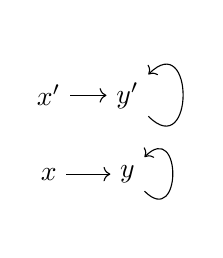
\begin{tikzpicture}
			\node (x) at (0, 0) {$x$};
			\node (y) at (1, 0) {$y$};
			\node (x') at (0, 1) {$x'$};
			\node (y') at (1, 1) {$y'$};
			\draw[->] (x) -- (y);
			\draw[->] (y) to [out=-45, in=45, looseness=4] (y);
			\draw[->] (x') -- (y');
			\draw[->] (y') to [out=-45, in=45, looseness=4] (y');
		\end{tikzpicture}
	\end{figure}
	从图中可以看出,$x$的后继闭包$\overline{x} = \{x, y\}$,$x'$的后继闭包$\overline{x'} = \{x', y'\}$。可以看出,$x$的后继闭包与$x'$的后继闭包无交。
\end{example}

\begin{example}
	考虑以下后继集合$(X, s)$:
	\begin{figure}[H]
		\centering
		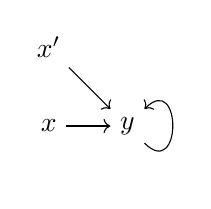
\begin{tikzpicture}
			\node (x) at (0, 0) {$x$};
			\node (y) at (1, 0) {$y$};
			\node (x') at (0, 1) {$x'$};
			\draw[->] (x) -- (y);
			\draw[->] (x') -- (y);
			\draw[->] (y) to [out=-45, in=45, looseness=4] (y);
		\end{tikzpicture}
	\end{figure}
	从图中可以看出,$x$的后继闭包$\overline{x} = \{x, y\}$,$x'$的后继闭包$\overline{x'} = \{x', y\}$。可以看出,$x$的后继闭包与$x'$的后继闭包有交,但没有包含关系。
\end{example}

\begin{example}
	考虑以下后继集合$(X, s)$:
	\begin{figure}[H]
		\centering
		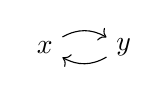
\begin{tikzpicture}
			\node (x) at (0, 0) {$x$};
			\node (y) at (1, 0) {$y$};
			\draw[->] (x) to[bend left] (y);
			\draw[->] (y) to[bend left] (x);
		\end{tikzpicture}
	\end{figure}
	从图中可以看出,$x$的后继闭包$\overline{x} = \{x, y\}$,$y$的后继闭包$\overline{y} = \{x, y\}$。可以看出,$x$的后继闭包与$y$的后继闭包相等。但$x$与$y$本身不相等。
\end{example}

上面的每个例子中,后继集合的元素个数都较少,目的是为了用最简单的例子来展示后继闭包之间的不同关系。实际上,可以在上面的例子中添加一些新的点,但它们之间关系的基本情况是差不多的。我们能看到,两个点的后继闭包,大体可以分为无交和有交两种情况,而有交的情况又可继续分为相等、真包含、不相包含这三种。对于后继闭包无交的两个点,看上去它们从属于两个不同的分支,而有交的两个点看上去则属于同一个分支。这个观察引出了一个猜测的方向:是否可以将后继集合中的点分为不同的分支,使得同一分支中的点的后继闭包相等,不同分支中的点的后继闭包无交?换句话说,这是在问“后继闭包有交”是否能导出集合的划分,也就是问它是否是一个等价关系。

借用拓扑的术语,我们定义两个点的不可分离性:

\begin{definition}[不可分离的点]
	对于后继集合$(X, s)$,$x, y \in X$,如果$x$的后继闭包$\overline{x}$与$y$的后继闭包$\overline{y}$满足:$y \in \overline{x} \vee x \in \overline{y}$,则称$x$与$y$是不可分离的。
\end{definition}



\subsection{第二步划分:不可区分的点类}

\end{document}